\subsection{Statistical analysis}
\label{sec:res-stats}

This subsection tests the main findings of Q1--Q3 with classical inference: first the 26 parameters of the step~9 group analysis
(\vn{crossing_ml_params.m}), then the variables and models of the machine-learning dataset (\vn{crossing_ml_stats.m};
Section~\ref{sec:analyses}). As in step~9, the leading and the trailing limb are analysed separately.

\subsubsection{The 26 parameters of the step 9 group analysis}
\label{sec:res-params}

Step~9 exports 26 parameters per limb and obstacle for SPSS: 5 clearance, 5 joint-angle, 6 segment-tilt, 7 peak-timing and 3
spatiotemporal parameters, as participant means. \vn{crossing_ml_params.m} tests all of them on the current sheet ($n = 10$). On the
sheet of the earlier SPSS run (26 October, $n = 9$) its repeated-measures ANOVA reproduces the SPSS GLM exactly: identical $F$ and
Greenhouse--Geisser $p$ in all 14 SPSS tables that were compared. Beyond the GLM it controls the false discovery rate (FDR) over the 52
parameter $\times$ limb tests of each effect, and adds the change per cm of obstacle, the comparison with level walking, rank-based
tests, a check without outlying cells, an equivalence test of the clearance and the detectable effect size (full tables in
Appendix~\ref{app:extra}).

\paragraph{What changes.} After the FDR correction, obstacle height changes 6 of the 26 parameters of each limb
(Table~\ref{tab:paramoverview}, Figure~\ref{fig:params}). The clearest are the Dot segment tilts of the limb that does the lifting: the
forward tilt and tilt ROM of the leading thigh (partial $\eta^2$ 0.87 and 0.89; +1.16\textdegree{} and +1.14\textdegree{} per cm of
obstacle) and the backward tilt and tilt ROM of the trailing shank (0.90 and 0.85; +1.23\textdegree{} and +1.13\textdegree{} per cm).
The hip ROM of both limbs, the leading knee peak flexion and ankle ROM, the trailing foot-tilt ROM, the trailing cadence and the gait
speed (about $-0.15$\,m/s from H1 to H3) also change. No clearance and no peak-timing parameter changes significantly with height.
Width changes only three leading-limb segment parameters (thigh forward tilt, thigh tilt ROM and shank tilt ROM; partial $\eta^2$
0.65--0.82); the shorter landing distance for the deeper obstacle (about 5\,cm, $p \leq 0.007$) does not survive the FDR correction,
and no parameter shows a height $\times$ width interaction. Against level walking, 10 (leading) and 14 (trailing) of the 21
parameters with a level-walk value change when an obstacle is crossed, 9 and 15 already at the lowest obstacle; the largest
differences are the leading thigh tilt ($d_z = 7.0$), the trailing shank tilt ($d_z = 3.8$), the stride length (+28 to +31\,cm) and
the cadence ($-14$ to $-19$ steps/min).

\begin{table}[htbp]
\centering
\caption{Step~9 parameters with a significant effect after the FDR correction (leading / trailing limb): height, width and their
interaction from the repeated-measures ANOVA, and the mean of the six obstacles against level walking.}
\label{tab:paramoverview}
\begin{adjustbox}{max width=\textwidth}
{\footnotesize
\begin{tabular}{lrrrrr}
\toprule
\textbf{class} & \textbf{parameters} & \textbf{height (lead / trail)} & \textbf{width (lead / trail)} & \textbf{height $\times$ width (lead / trail)} & \textbf{obstacles vs level walk (lead / trail)} \\
\midrule
clearance (camera) & 5 & 0 / 0 & 0 / 0 & 0 / 0 & - (no level walk) \\
joint angles (IK) & 5 & 3 / 1 & 0 / 0 & 0 / 0 & 2 / 5 of 5 \\
segment tilts (Dot) & 6 & 2 / 3 & 3 / 0 & 0 / 0 & 5 / 5 of 6 \\
peak timing (vs clearance) & 7 & 0 / 0 & 0 / 0 & 0 / 0 & 1 / 2 of 7 \\
spatiotemporal & 3 & 1 / 2 & 0 / 0 & 0 / 0 & 2 / 2 of 3 \\
\textbf{all} & 26 & 6 / 6 & 3 / 0 & 0 / 0 & 10 / 14 of 21 \\
\bottomrule
\end{tabular}
}
\end{adjustbox}

\end{table}

\begin{figure}[htbp]
\centering
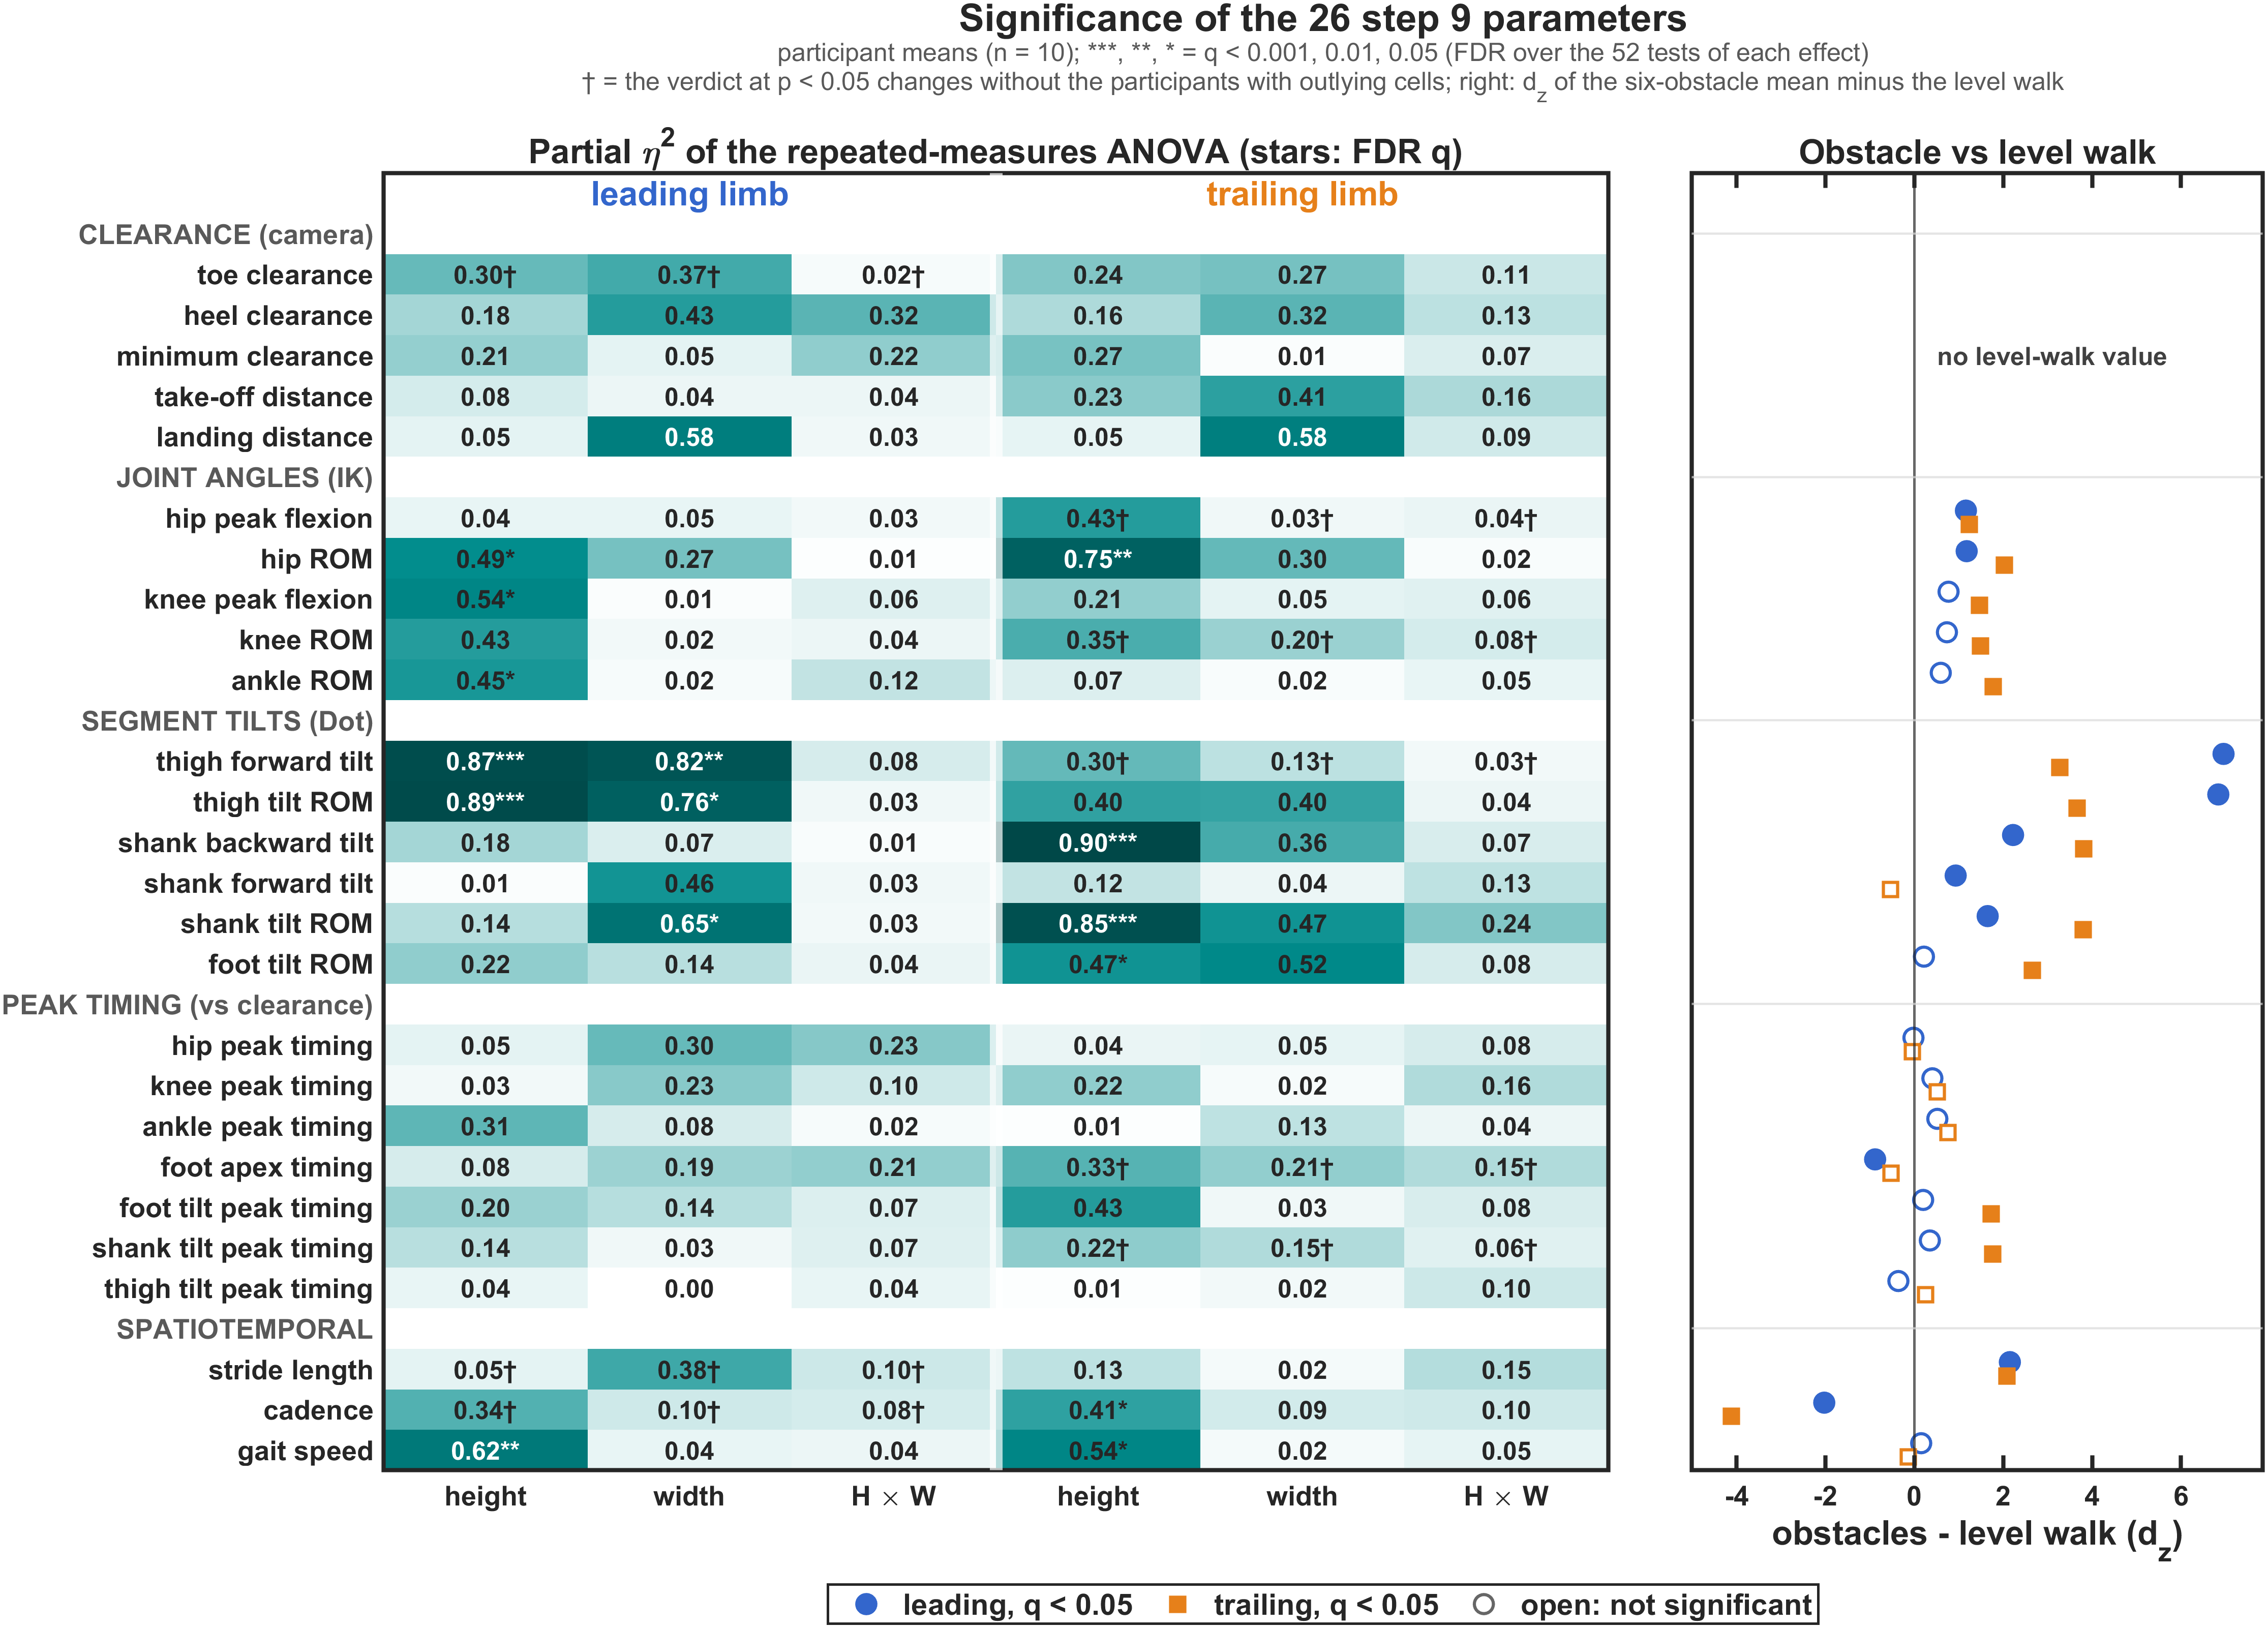
\includegraphics[width=\textwidth]{fig_params.png}
\caption{Significance of the 26 step~9 parameters (participant means, $n = 10$). Left: partial $\eta^2$ of the repeated-measures
ANOVA for height, width and their interaction, leading and trailing limb; ***, **, * = FDR $q < 0.001$, 0.01, 0.05 over the 52 tests
of each effect; $\dagger$ = the verdict at $p < 0.05$ changes without the participants with outlying cells. Right: effect size $d_z$
of the mean of the six obstacles minus the level walk (filled = $q < 0.05$; the clearance has no level-walk value).}
\label{fig:params}
\end{figure}

\paragraph{Is the clearance kept constant?} A non-significant test with ten people does not show that nothing changes, so the
clearance was also tested for equivalence (Table~\ref{tab:paramclear}, Figure~\ref{fig:paramsclear}). From H1 to H3 the obstacle
rises by 18.5\,cm, while the minimum clearance of the leading limb changes by $-1.2$\,cm (90\,\% CI $-2.6$ to $+0.3$): changes beyond
2.6\,cm, 14\,\% of the obstacle rise, are excluded (two one-sided tests, $\alpha = 0.05$), so the leading foot keeps its clearance.
The minimum clearance of the trailing limb falls by 3.5\,cm (90\,\% CI $-6.9$ to $-0.2$) and a change of up to 6.9\,cm cannot be
excluded: for the trailing foot a constant clearance is not shown. The toe and heel clearances give bounds of 5.6 / 7.0 and
2.3 / 6.6\,cm (leading / trailing).

\begin{table}[htbp]
\centering
\caption{Clearance class: change from H1 to H3 and from W1 to W2 (90\,\% CI) and the bound beyond which a change is excluded (two
one-sided tests, $\alpha = 0.05$).}
\label{tab:paramclear}
\begin{adjustbox}{max width=\textwidth}
{\footnotesize
\begin{tabular}{llrlrlr}
\toprule
\textbf{parameter} & \textbf{limb} & \textbf{n} & \textbf{H3 - H1 (90 \% CI), cm} & \textbf{bound} & \textbf{W2 - W1 (90 \% CI), cm} & \textbf{bound} \\
\midrule
toe clearance & lead & 10 & $-$3.1 ($-$5.6 to $-$0.6) & 5.6 & +3.4 (+0.7 to +6.1) & 6.1 \\
toe clearance & trail & 10 & $-$3.5 ($-$7.0 to +0.1) & 7.0 & +3.1 ($-$0.0 to +6.3) & 6.3 \\
heel clearance & lead & 10 & $-$0.8 ($-$2.3 to +0.6) & 2.3 & +2.7 (+0.8 to +4.6) & 4.6 \\
heel clearance & trail & 10 & $-$2.9 ($-$6.6 to +0.9) & 6.6 & +3.1 (+0.3 to +5.8) & 5.8 \\
minimum clearance & lead & 10 & $-$1.2 ($-$2.6 to +0.3) & 2.6 & +0.7 ($-$1.1 to +2.4) & 2.4 \\
minimum clearance & trail & 10 & $-$3.5 ($-$6.9 to $-$0.2) & 6.9 & +0.6 ($-$2.9 to +4.1) & 4.1 \\
take-off distance & lead & 10 & $-$2.7 ($-$5.8 to +0.5) & 5.8 & $-$1.3 ($-$5.4 to +2.8) & 5.4 \\
take-off distance & trail & 10 & $-$3.6 ($-$6.9 to $-$0.4) & 6.9 & $-$2.8 ($-$4.8 to $-$0.7) & 4.8 \\
landing distance & lead & 10 & $-$3.4 ($-$12.1 to +5.3) & 12.1 & $-$5.4 ($-$8.1 to $-$2.6) & 8.1 \\
landing distance & trail & 10 & $-$1.0 ($-$7.8 to +5.8) & 7.8 & $-$5.2 ($-$7.9 to $-$2.5) & 7.9 \\
\bottomrule
\end{tabular}
}
\end{adjustbox}

\end{table}

\begin{figure}[htbp]
\centering
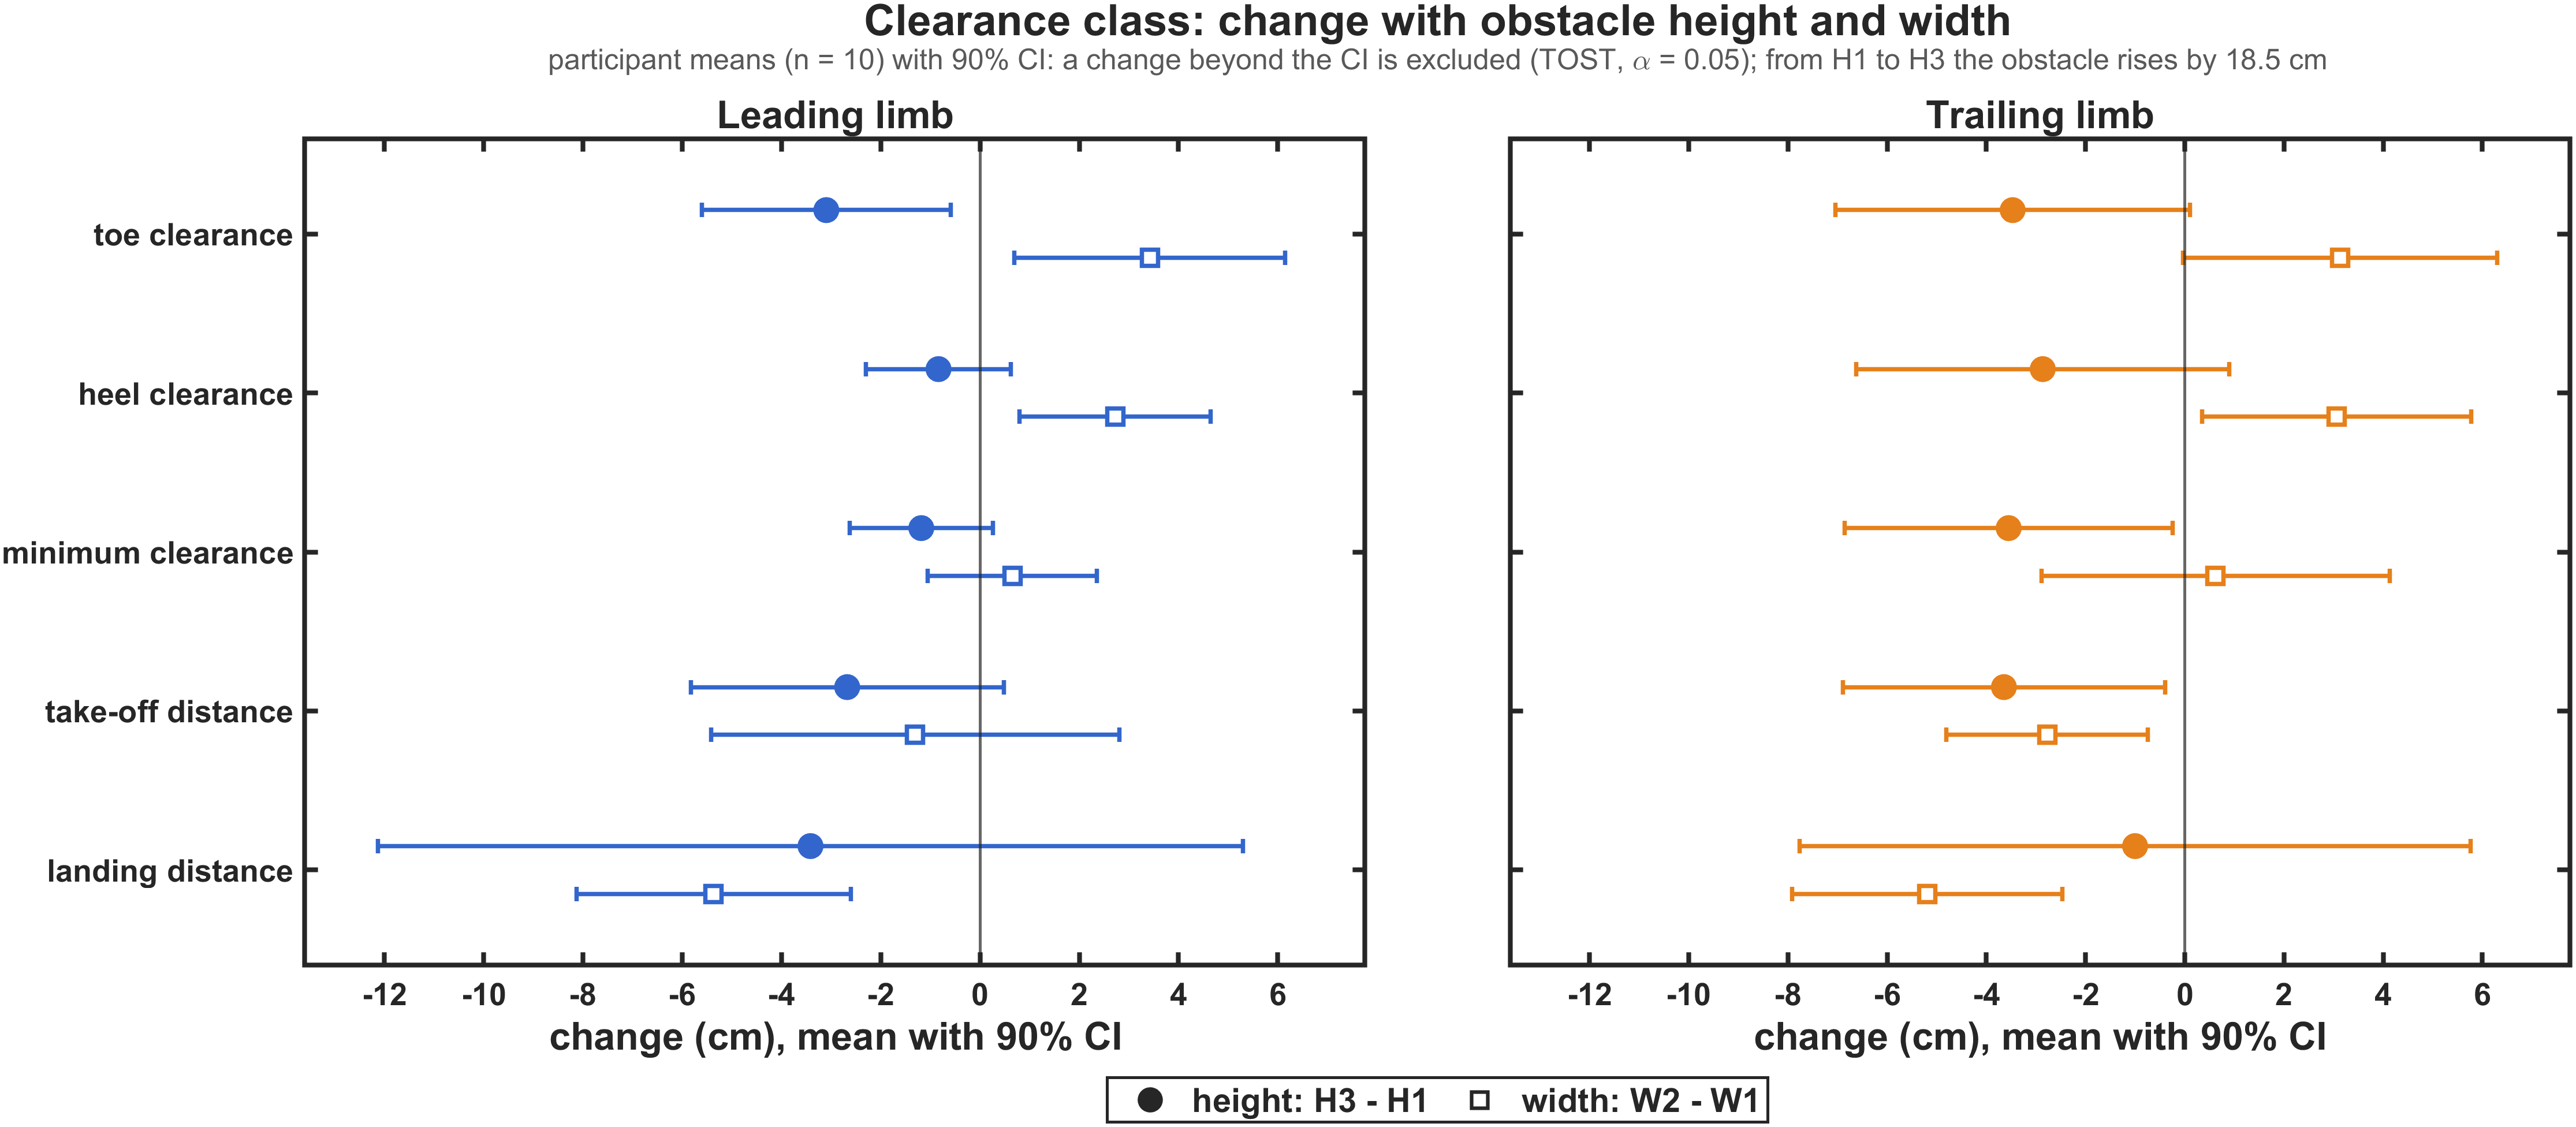
\includegraphics[width=\textwidth]{fig_params_clear.png}
\caption{Clearance class: change of the participant means from H1 to H3 (filled) and from W1 to W2 (open) with the 90\,\% CI, leading
(left) and trailing limb (right). A change beyond the CI is excluded by two one-sided tests ($\alpha = 0.05$); from H1 to H3 the
obstacle rises by 18.5\,cm.}
\label{fig:paramsclear}
\end{figure}

\paragraph{Robustness and cells to check.} Rank-based tests give the same verdict as the ANOVA for 43 of the 52 height effects
(Friedman) and 49 of the 52 width effects (Wilcoxon; Table~\ref{tab:paramnonpar}). 93 of the 3120 participant means are outlying
(modified $z$-score above 3.5 within their obstacle column; Table~\ref{tab:paramoutliers}), 42 of them in the IK joint angles and 28 in
the peak timings. Some cannot be real angles: participant 104's leading-limb knee ROM of 238--274\textdegree{} and hip peak flexion of
123--157\textdegree{} (column medians 60--80\textdegree{} and 37--50\textdegree{}) point to an IK processing artefact. Others, such as
participant 101's trailing shank-tilt peak timing of +11.5\,\% of the gait cycle at W2\_H2 (column median $-3.0$\,\%), may be a jump
of the peak detection to another maximum. Without the participants with outlying cells the verdict at $p < 0.05$ changes for 8
parameter $\times$ limb combinations (Table~\ref{tab:paramsens}, $\dagger$ in Figure~\ref{fig:params}); the height effect on the
trailing shank-tilt peak timing, for example, goes from $p = 0.143$ to $p < 0.001$. These cells should be checked in step~9 (for the
joint angles, e.g.\ with \vn{manualJointValues.m}) before the joint-angle and timing tests, here and in SPSS, are interpreted; no value
was changed for this analysis.

\paragraph{How large an effect ten people can detect.} With 10 participants a paired comparison detects (80\,\% power,
$\alpha = 0.05$) only effects of $d_z \geq 1.0$. Of the 70 height and width contrasts that are not significant, 54 have
$\lvert d_z \rvert < 0.5$ and would need more than 34 participants; the largest of them ($\lvert d_z \rvert \approx 0.7$: the trailing
shank backward tilt with width and the leading cadence with height) would need 18--19. A non-significant step~9 parameter in this study
therefore means ``no large effect'', not ``no effect''.

\subsubsection{Foot lift and clearance in the machine-learning dataset}

In the repeated-measures ANOVA of the participant means (Table~\ref{tab:anova}, Figure~\ref{fig:stats}), obstacle height changes the
Dot foot lift, the
leading-thigh flexion, the trailing-shank heel-up and the trailing swing time (partial $\eta^2$ 0.37--0.97, all
$p \leq 0.043$), but neither the leading swing time nor the camera minimum clearance of either limb. Every pair of height levels
differs for the foot lift and the segment angles (Holm $p \leq 0.001$, $\lvert d_z \rvert$ 1.5--7.1; Table~\ref{tab:contrasts}).
Width also shifts the foot lift, the leading-thigh flexion, the trailing-shank heel-up and the trailing swing time
($p \leq 0.044$), and no variable shows a height $\times$ width interaction.

The mixed models on every crossing (Table~\ref{tab:statlme}) add the width and the repeat to the height model of
Section~\ref{sec:res-biomech} and leave its slopes unchanged: the foot rises by 10.1\,mm (leading) and 11.1\,mm (trailing) per cm
of obstacle, the leading thigh flexes 1.2\textdegree{} more and the trailing shank tilts back 1.2\textdegree{} more per cm, and
the camera clearance does not change significantly ($-0.7$ and $-2.3$\,mm per cm, $p \geq 0.06$). A 15\,cm deep obstacle raises
the foot by 25\,mm compared with a 5\,cm one of the same height: as much as 2.3--2.5\,cm of extra obstacle height, and well below
the crossing-to-crossing SD of about 40\,mm. This reconciles the significant width effect with the near-chance width recognition
(Section~\ref{sec:res-width}): the shift is consistent across people, and therefore significant for the group means, but too small
against the variation of single crossings to recognise the width of one obstacle. The foot lift shows no significant linear trend
over the five repeats of an obstacle; the higher first crossing of Section~\ref{sec:res-biomech} is a single step, which a linear
trend captures poorly. Only the trailing-shank heel-up changes slightly over the repeats (+0.65\textdegree{} per repeat,
$p = 0.037$).

\begin{table}[htbp]
\centering
\caption{Repeated-measures ANOVA, height (3) $\times$ width (2), on the participant means of each limb separately
(Greenhouse--Geisser $p$; partial $\eta^2$).}
\label{tab:anova}
\begin{adjustbox}{max width=\textwidth}
{\scriptsize
\begin{tabular}{llrp{3.5cm}p{3.5cm}p{3.5cm}}
\toprule
\textbf{limb} & \textbf{variable} & \textbf{n} & \textbf{height: F (df), p, partial $\eta^2$} & \textbf{width: F (df), p, partial $\eta^2$} & \textbf{height $\times$ width: F (df), p, partial $\eta^2$} \\
\midrule
lead & foot lift (Dot) (mm) & 10 & F(2, 18) = 260.5, p $<$ 0.001, 0.97 & F(1, 9) = 35.6, p $<$ 0.001, 0.80 & F(2, 18) = 0.6, p = 0.552, 0.06 \\
lead & thigh flexion (Dot) (deg) & 10 & F(2, 18) = 73.4, p $<$ 0.001, 0.89 & F(1, 9) = 21.4, p = 0.001, 0.70 & F(2, 18) = 2.0, p = 0.186, 0.18 \\
lead & swing time (Dot) (s) & 10 & F(2, 18) = 1.9, p = 0.194, 0.17 & F(1, 9) = 1.1, p = 0.330, 0.11 & F(2, 18) = 1.1, p = 0.352, 0.11 \\
lead & minimum clearance (camera) (mm) & 10 & F(2, 18) = 2.3, p = 0.148, 0.20 & F(1, 9) = 0.5, p = 0.497, 0.05 & F(2, 18) = 2.0, p = 0.173, 0.18 \\
trail & foot lift (Dot) (mm) & 10 & F(2, 18) = 121.2, p $<$ 0.001, 0.93 & F(1, 9) = 28.7, p $<$ 0.001, 0.76 & F(2, 18) = 1.6, p = 0.241, 0.15 \\
trail & shank heel-up (Dot) (deg) & 10 & F(2, 18) = 57.2, p $<$ 0.001, 0.86 & F(1, 9) = 5.5, p = 0.044, 0.38 & F(2, 18) = 1.5, p = 0.261, 0.14 \\
trail & swing time (Dot) (s) & 10 & F(2, 18) = 5.2, p = 0.043, 0.37 & F(1, 9) = 8.3, p = 0.018, 0.48 & F(2, 18) = 3.9, p = 0.054, 0.30 \\
trail & minimum clearance (camera) (mm) & 10 & F(2, 18) = 3.0, p = 0.098, 0.25 & F(1, 9) = 0.1, p = 0.740, 0.01 & F(2, 18) = 0.7, p = 0.488, 0.07 \\
\bottomrule
\end{tabular}
}
\end{adjustbox}

\end{table}

\begin{table}[htbp]
\centering
\caption{Height contrasts: difference of the participant means averaged over width, $d_z$ and Holm-corrected $p$.}
\label{tab:contrasts}
\begin{adjustbox}{max width=\textwidth}
{\scriptsize
\begin{tabular}{llp{3.4cm}p{3.4cm}p{3.4cm}}
\toprule
\textbf{limb} & \textbf{variable} & \textbf{H2 - H1} & \textbf{H3 - H2} & \textbf{H3 - H1} \\
\midrule
lead & foot lift (Dot) (mm) & +105 (dz 3.5, p $<$ 0.001) & +81 (dz 4.0, p $<$ 0.001) & +186 (dz 7.1, p $<$ 0.001) \\
lead & thigh flexion (Dot) (deg) & +14.1 (dz 1.9, p $<$ 0.001) & +7.7 (dz 2.7, p $<$ 0.001) & +21.8 (dz 3.7, p $<$ 0.001) \\
lead & swing time (Dot) (s) & +0.031 (dz 0.5, p = 0.401) & +0.012 (dz 0.2, p = 0.587) & +0.043 (dz 0.5, p = 0.401) \\
lead & minimum clearance (camera) (mm) & +7 (dz 0.2, p = 0.544) & $-$18 (dz $-$1.1, p = 0.026) & $-$11 (dz $-$0.4, p = 0.544) \\
trail & foot lift (Dot) (mm) & +114 (dz 5.3, p $<$ 0.001) & +92 (dz 1.9, p $<$ 0.001) & +206 (dz 4.1, p $<$ 0.001) \\
trail & shank heel-up (Dot) (deg) & $-$13.1 (dz $-$3.4, p $<$ 0.001) & $-$8.9 (dz $-$1.5, p = 0.001) & $-$22.0 (dz $-$2.5, p $<$ 0.001) \\
trail & swing time (Dot) (s) & +0.016 (dz 0.8, p = 0.078) & +0.028 (dz 0.6, p = 0.080) & +0.044 (dz 0.8, p = 0.078) \\
trail & minimum clearance (camera) (mm) & $-$15 (dz $-$0.4, p = 0.297) & $-$28 (dz $-$0.5, p = 0.297) & $-$43 (dz $-$0.6, p = 0.258) \\
\bottomrule
\end{tabular}
}
\end{adjustbox}

\end{table}

\begin{table}[htbp]
\centering
\caption{Mixed models on every crossing: height slope (mean over the widths), width effect at the mean height, difference of the
slopes, repeat trend (95\,\% CI, Satterthwaite $p$), residual SD and $R^2$ (marginal / conditional).}
\label{tab:statlme}
\begin{adjustbox}{max width=\textwidth}
{\scriptsize
\begin{tabular}{llp{2.5cm}p{2.5cm}p{2.5cm}p{2.5cm}rr}
\toprule
\textbf{limb} & \textbf{variable} & \textbf{per cm of height} & \textbf{W2 vs W1} & \textbf{slope W2 - W1 (per cm)} & \textbf{per repeat} & \textbf{residual SD} & \textbf{$R^2$ m / c} \\
\midrule
lead & foot lift (Dot) (mm) & +10.1 (+9.4 to +10.7), p $<$ 0.001 & +25.1 (+15.1 to +35.2), p $<$ 0.001 & $-$0.2 ($-$1.5 to +1.1), p = 0.735 & $-$0.8 ($-$4.3 to +2.8), p = 0.676 & 40.9 & 0.52 / 0.86 \\
lead & thigh flexion (Dot) (deg) & +1.20 (+1.02 to +1.37), p $<$ 0.001 & +3.44 (+1.97 to +4.91), p $<$ 0.001 & $-$0.25 ($-$0.44 to $-$0.06), p = 0.011 & +0.44 ($-$0.08 to +0.96), p = 0.096 & 5.98 & 0.47 / 0.82 \\
lead & swing time (Dot) (s) & +0.0024 ($-$0.0006 to +0.0055), p = 0.106 & $-$0.0155 ($-$0.0359 to +0.0048), p = 0.133 & $-$0.0008 ($-$0.0034 to +0.0019), p = 0.567 & +0.0021 ($-$0.0051 to +0.0093), p = 0.564 & 0.0828 & 0.02 / 0.63 \\
lead & minimum clearance (camera) (mm) & $-$0.7 ($-$1.8 to +0.4), p = 0.183 & +6.2 ($-$3.8 to +16.3), p = 0.224 & +1.1 ($-$0.2 to +2.4), p = 0.106 & +0.2 ($-$3.3 to +3.8), p = 0.904 & 41.0 & 0.01 / 0.55 \\
trail & foot lift (Dot) (mm) & +11.1 (+9.6 to +12.6), p $<$ 0.001 & +25.4 (+15.6 to +35.3), p $<$ 0.001 & +1.3 ($-$0.0 to +2.5), p = 0.054 & $-$2.4 ($-$5.8 to +1.1), p = 0.182 & 40.1 & 0.51 / 0.89 \\
trail & shank heel-up (Dot) (deg) & $-$1.19 ($-$1.49 to $-$0.89), p $<$ 0.001 & $-$2.78 ($-$4.51 to $-$1.05), p = 0.002 & $-$0.15 ($-$0.37 to +0.08), p = 0.195 & +0.65 (+0.04 to +1.26), p = 0.037 & 7.05 & 0.28 / 0.83 \\
trail & swing time (Dot) (s) & +0.0024 (+0.0002 to +0.0045), p = 0.033 & +0.0147 (+0.0059 to +0.0235), p = 0.001 & +0.0012 (+0.0001 to +0.0024), p = 0.035 & +0.0017 ($-$0.0014 to +0.0048), p = 0.279 & 0.0358 & 0.08 / 0.61 \\
trail & minimum clearance (camera) (mm) & $-$2.3 ($-$4.7 to +0.1), p = 0.060 & +4.2 ($-$14.8 to +23.2), p = 0.662 & +2.0 ($-$0.5 to +4.5), p = 0.114 & +0.6 ($-$6.1 to +7.3), p = 0.851 & 77.3 & 0.04 / 0.47 \\
\bottomrule
\end{tabular}
}
\end{adjustbox}

\end{table}

\begin{figure}[htbp]
\centering
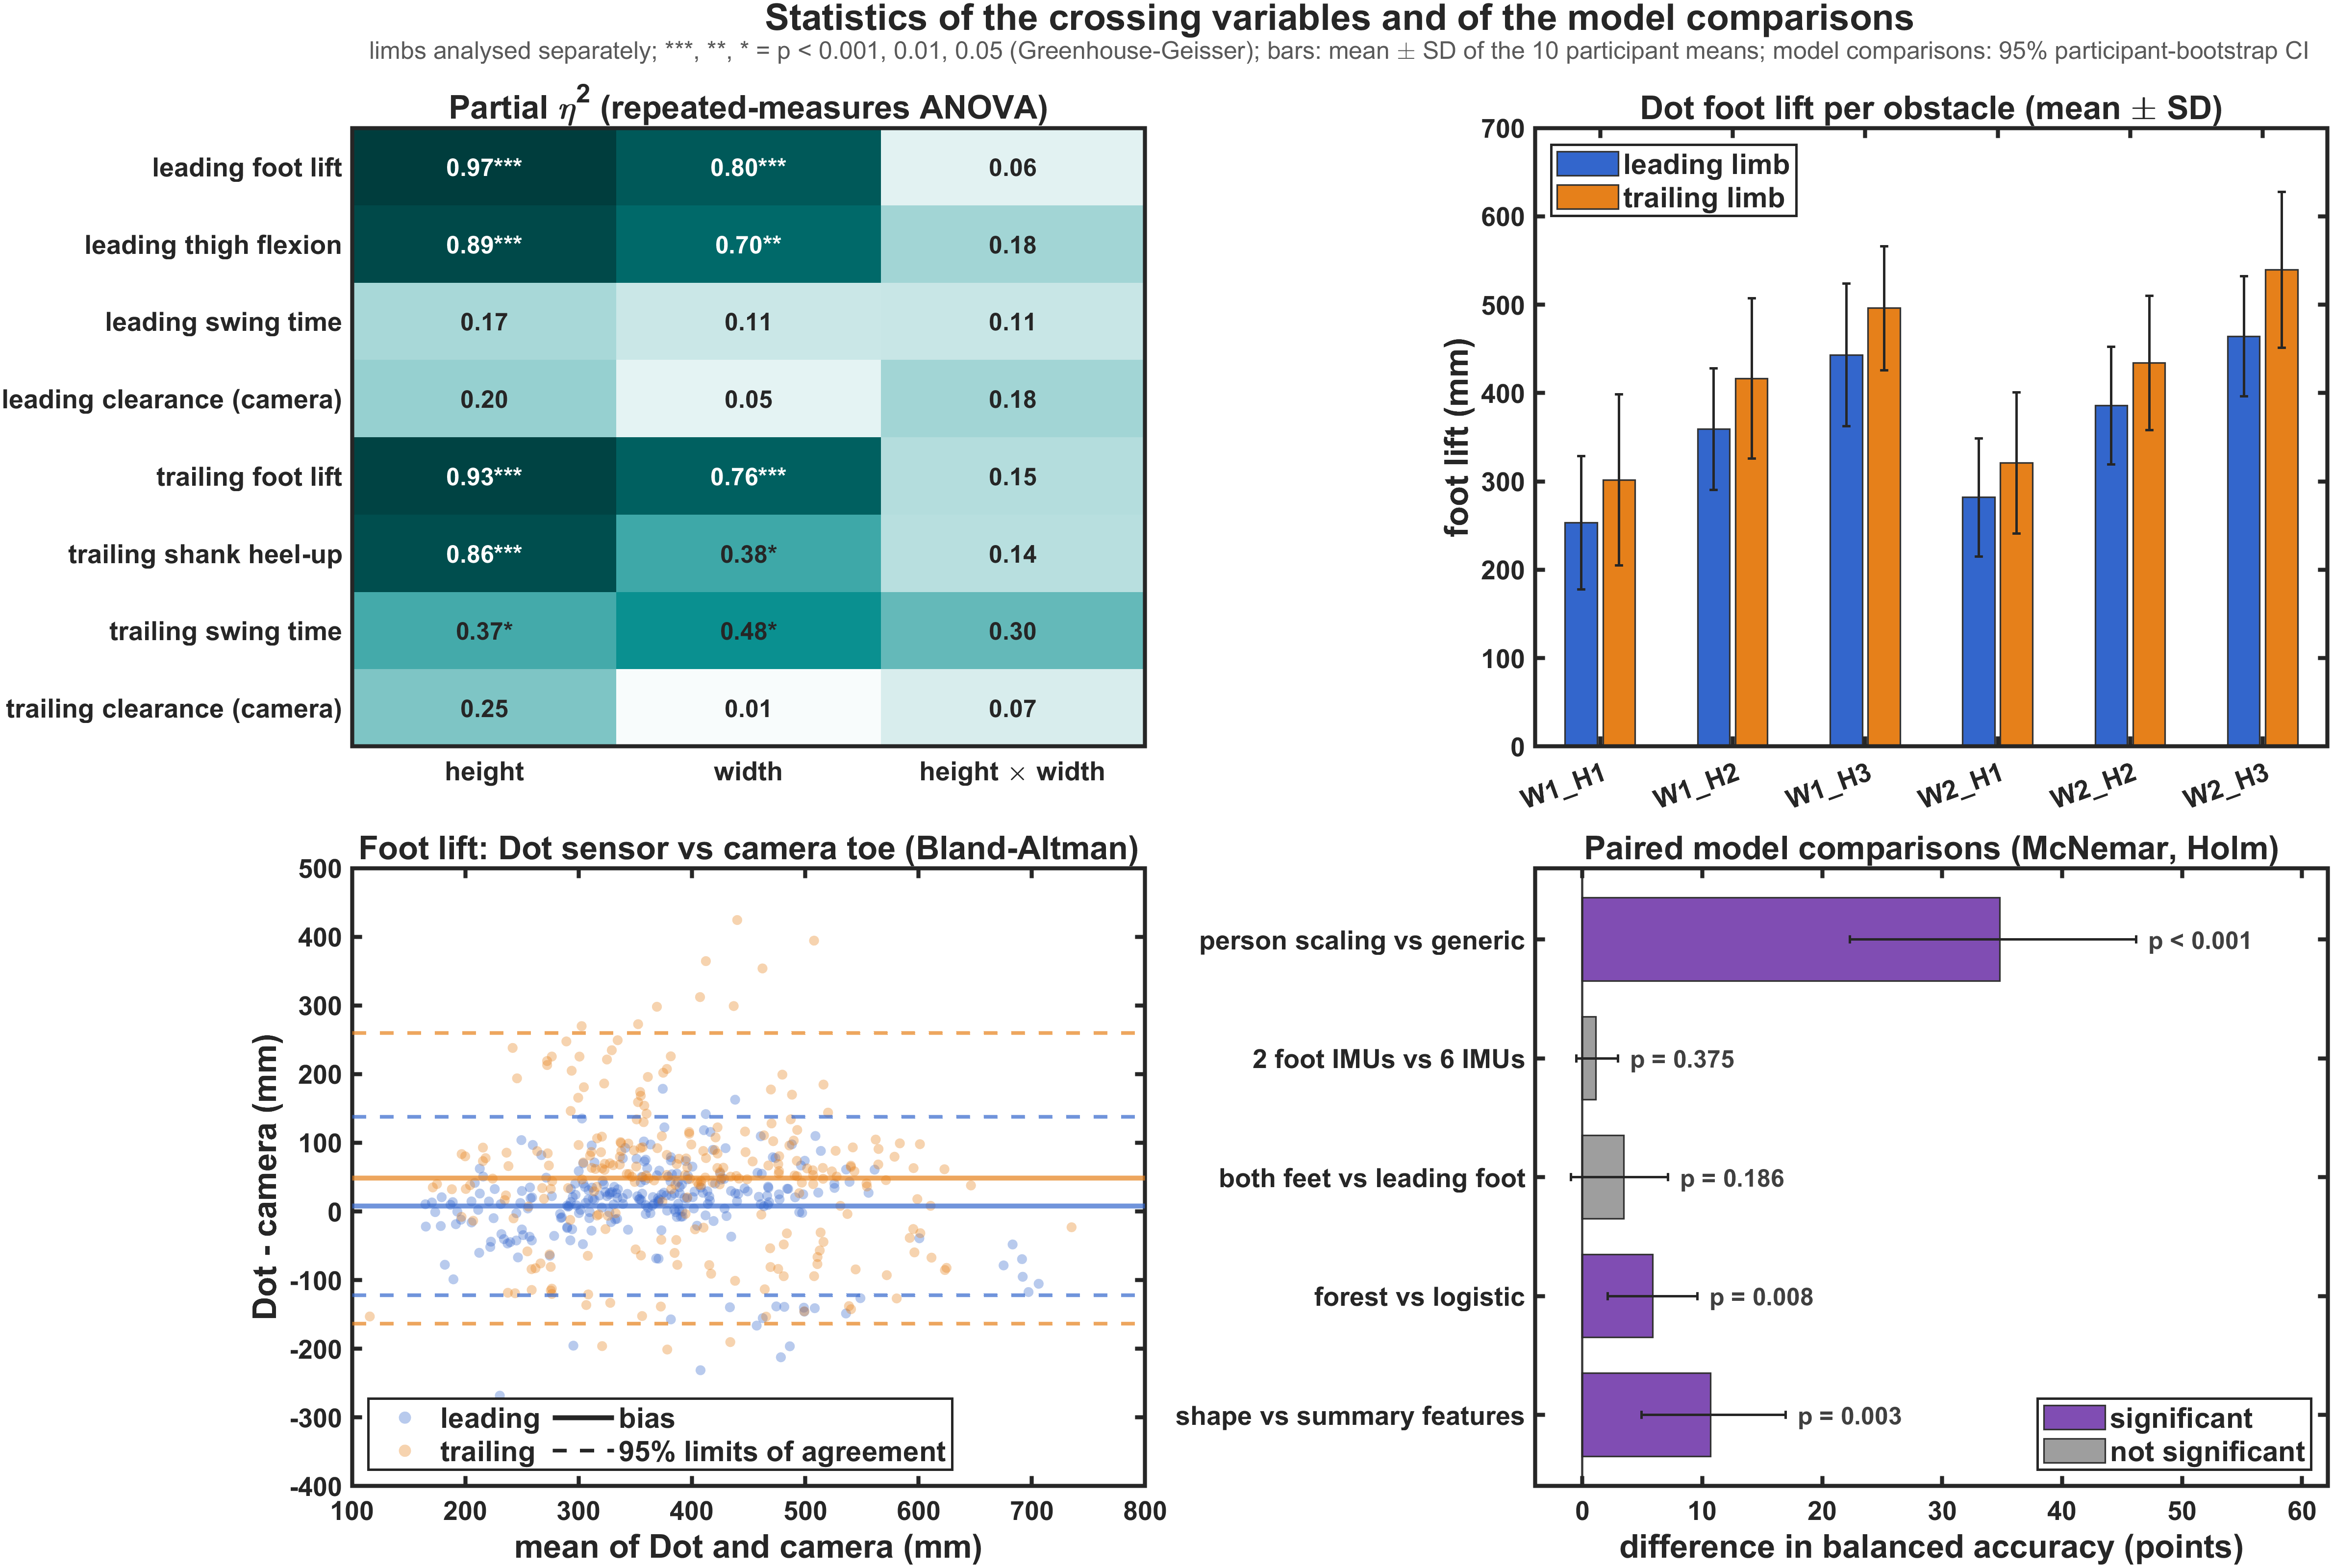
\includegraphics[width=\textwidth]{fig_stats.png}
\caption{Statistics. Top left: partial $\eta^2$ of height, width and their interaction for each limb and variable (stars:
Greenhouse--Geisser $p$). Top right: Dot foot lift per obstacle, leading (blue) and trailing (orange) limb, mean $\pm$ SD of the
participant means. Bottom left: Bland--Altman plot of the Dot foot lift against the camera toe rise (solid = bias, dashed = 95\,\%
limits of agreement). Bottom right: paired model comparisons, difference in balanced accuracy with 95\,\% participant-bootstrap CI
and Holm-corrected McNemar $p$ (purple = significant).}
\label{fig:stats}
\end{figure}

\subsubsection{Agreement of the IMU with the camera}

The rise of the Dot foot sensor differs from the camera toe rise by a mean of $+8$\,mm (leading) and $+48$\,mm (trailing), with
wide limits of agreement ($-122$ to $+137$ and $-163$ to $+260$\,mm) and no proportional bias (Table~\ref{tab:agreement},
Figure~\ref{fig:stats}). The sensor on the dorsum and the marker on the toe follow different points of a foot that rotates during
the crossing, so the toe height of a single crossing cannot be read from the foot sensor; this is the measurement side of the
clearance result (Section~\ref{sec:res-clearance}). The IMU toe-off event comes a median 83\,ms (leading) and 233\,ms (trailing)
after the camera lift-off, and for the trailing limb the delay grows by 4.9\,ms per cm of obstacle ($p < 0.001$); every timing
in the haptic analyses therefore uses the camera lift-off.

\begin{table}[htbp]
\centering
\caption{Agreement of the IMU with the camera: foot lift (Dot sensor rise minus camera toe rise; Bland--Altman) and toe-off time
(IMU step-4 toe-off minus camera lift-off).}
\label{tab:agreement}
\begin{adjustbox}{max width=\textwidth}
{\scriptsize
\begin{tabular}{lrrrrrrrr}
\toprule
\textbf{limb} & \textbf{n} & \textbf{foot lift: bias (mm)} & \textbf{LoA (mm)} & \textbf{proportional bias (mm per mm)} & \textbf{toe-off: bias (ms)} & \textbf{LoA (ms)} & \textbf{median (IQR)} & \textbf{per cm of obstacle} \\
\midrule
lead & 260 & +8 & $-$122 to +137 & $-$0.02 (p = 0.600) & +106 & $-$134 to +345 & +83 (+17 to +167) & $-$0.6 ms (p = 0.436) \\
trail & 259 & +48 & $-$163 to +260 & $-$0.07 (p = 0.280) & +272 & $-$5 to +548 & +233 (+167 to +367) & +4.9 ms (p $<$ 0.001) \\
\bottomrule
\end{tabular}
}
\end{adjustbox}

\end{table}

\subsubsection{Which model differences are real}

On the same 260 crossings (Tables~\ref{tab:statmodels} and \ref{tab:statpairs}), person scaling beats the generic model by 34.8
points (95\,\% CI 22.3--46.2; McNemar $p < 0.001$, Wilcoxon $p = 0.039$), the forest beats logistic regression by 5.9 points
($p = 0.008$) and the clearance-shape features beat the summary features in the generic model by 10.7 points ($p = 0.003$; all
Holm-corrected). The two foot IMUs are not worse than all six IMUs (1.1 points higher, $p = 0.38$), and the trailing foot adds
3.5 points to the leading foot without reaching significance ($p = 0.19$). Two foot IMUs are therefore sufficient, and the
decisive design choice is the person scaling. Cohen's $\kappa$ is 0.88 for the device model and 0.36 for the generic one. The
Wilcoxon test on the ten participant accuracies has little power (its smallest possible $p$ is 0.002) and confirms only the
person scaling.

\begin{table}[htbp]
\centering
\caption{The main models on the same crossings: balanced accuracy (95\,\% CI), macro F1 and Cohen's $\kappa$.}
\label{tab:statmodels}
\begin{adjustbox}{max width=\textwidth}
{\footnotesize
\begin{tabular}{p{7.4cm}rrr}
\toprule
\textbf{model} & \textbf{balanced accuracy (95 \% CI)} & \textbf{macro F1} & \textbf{kappa} \\
\midrule
generic, forest vote, 2 foot IMUs & 57.5\% (47--70) & 0.56 & 0.36 \\
person scaling, forest vote, 2 foot IMUs (device) & 92.3\% (87--96) & 0.92 & 0.88 \\
person scaling, forest vote, 6 IMUs & 91.2\% (86--96) & 0.91 & 0.87 \\
person scaling, forest, leading foot only & 88.8\% (85--93) & 0.89 & 0.83 \\
person scaling, logistic vote, 2 foot IMUs & 86.4\% (81--92) & 0.87 & 0.80 \\
generic, logistic, leading summary features & 62.1\% (55--70) & 0.62 & 0.43 \\
generic, logistic, leading clearance-shape features & 72.8\% (65--80) & 0.71 & 0.59 \\
\bottomrule
\end{tabular}
}
\end{adjustbox}

\end{table}

\begin{table}[htbp]
\centering
\caption{Paired comparisons: difference in balanced accuracy (participant-bootstrap CI), crossings right for only one of the two
models, McNemar and Wilcoxon $p$ (Holm over the five pairs).}
\label{tab:statpairs}
\begin{adjustbox}{max width=\textwidth}
{\footnotesize
\begin{tabular}{p{5.4cm}rrrr}
\toprule
\textbf{comparison} & \textbf{difference (points, 95 \% CI)} & \textbf{only A right / only B right} & \textbf{McNemar p (Holm)} & \textbf{Wilcoxon p (Holm)} \\
\midrule
person scaling vs generic (forest vote, 2 foot IMUs) & +34.8 (+22.3 to +46.2) & 100 / 8 & p $<$ 0.001 & p = 0.039 \\
2 foot IMUs vs 6 IMUs (person scaling) & +1.1 ($-$0.5 to +3.0) & 4 / 1 & p = 0.375 & p = 0.625 \\
both feet vs leading foot only (person scaling) & +3.5 ($-$1.0 to +7.2) & 16 / 7 & p = 0.186 & p = 0.438 \\
forest vs logistic (person scaling) & +5.9 (+2.1 to +9.6) & 19 / 4 & p = 0.008 & p = 0.234 \\
clearance-shape vs summary features (generic, leading) & +10.7 (+4.9 to +16.9) & 44 / 17 & p = 0.003 & p = 0.078 \\
\bottomrule
\end{tabular}
}
\end{adjustbox}

\end{table}

\subsubsection{Leg dominance}

The dominant leg led 43.5\,\% of the crossings, and every participant but one (104) led with both legs at times. When the dominant
leg leads, the leading foot rises 21\,mm less, the leading thigh flexes 5.4\textdegree{} less and the leading clearance is 34\,mm
smaller; at the same time the trailing, non-dominant leg tilts its shank 2.6\textdegree{} further back and clears the obstacle by
46\,mm more (Table~\ref{tab:dominance}). The non-dominant leg thus crosses with the larger margin in either role. The device model
is right in 95.6\,\% of the crossings led by the dominant leg and 89.8\,\% of the others, not a significant difference (Fisher
$p = 0.10$), so the device can work without knowing which leg is dominant. Because the participants chose their leading leg,
these differences are associations, not effects of dominance alone.

\begin{table}[htbp]
\centering
\caption{Crossings led by the dominant minus the non-dominant leg (mixed models with height, width and a random height slope;
95\,\% CI, Satterthwaite $p$). For the trailing variables, the trailing leg is then the non-dominant one.}
\label{tab:dominance}
\begin{adjustbox}{max width=\textwidth}
{\footnotesize
\begin{tabular}{llrr}
\toprule
\textbf{limb} & \textbf{variable} & \textbf{dominant-led minus non-dominant-led (95 \% CI)} & \textbf{p} \\
\midrule
lead & foot lift (Dot) (mm) & $-$21.2 ($-$32.3 to $-$10.1) & p $<$ 0.001 \\
lead & thigh flexion (Dot) (deg) & $-$5.42 ($-$7.01 to $-$3.83) & p $<$ 0.001 \\
lead & swing time (Dot) (s) & $-$0.0072 ($-$0.0305 to +0.0162) & p = 0.546 \\
lead & minimum clearance (camera) (mm) & $-$34.4 ($-$45.1 to $-$23.8) & p $<$ 0.001 \\
trail & foot lift (Dot) (mm) & +5.0 ($-$6.5 to +16.6) & p = 0.390 \\
trail & shank heel-up (Dot) (deg) & $-$2.55 ($-$4.56 to $-$0.53) & p = 0.013 \\
trail & swing time (Dot) (s) & +0.0022 ($-$0.0081 to +0.0125) & p = 0.670 \\
trail & minimum clearance (camera) (mm) & +46.0 (+24.8 to +67.2) & p $<$ 0.001 \\
\bottomrule
\end{tabular}
}
\end{adjustbox}

\end{table}
